
%(BEGIN_QUESTION)
% Copyright 2009, Tony R. Kuphaldt, released under the Creative Commons Attribution License (v 1.0)
% This means you may do almost anything with this work of mine, so long as you give me proper credit

\vbox{\hrule \hbox{\strut \vrule{} {\bf Desktop Process exercise} \vrule} \hrule}

Set up one of the Desktop Process units to experiment with:

$$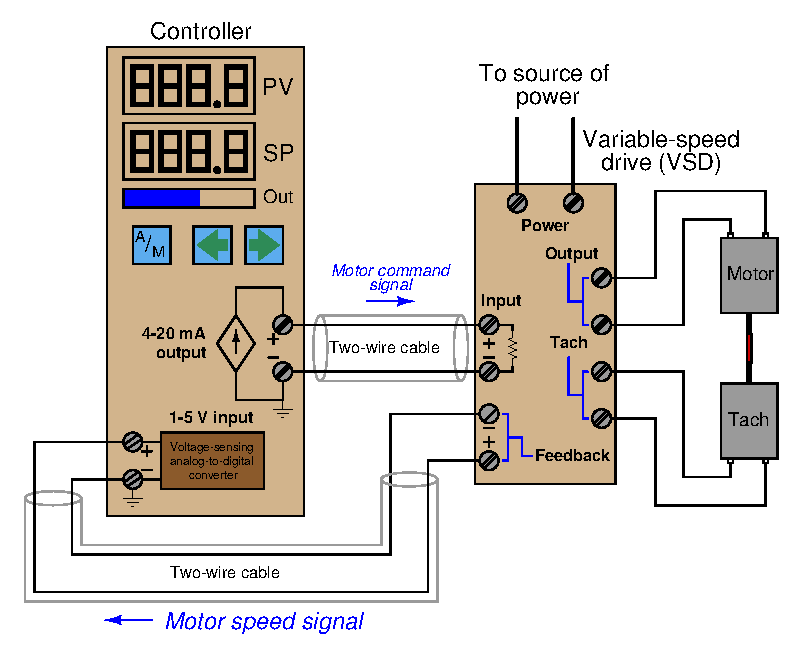
\includegraphics[width=15.5cm]{i04262x01.eps}$$

With the controller in manual mode, you should be able to drive the motor to different speeds, and see those speeds reflected as percentage values on the controller's process variable (PV) display.

\vskip 10pt

\noindent
Now, configure the controller as follows:

\begin{itemize}
\item{} Control action = {\it reverse}
\item{} Gain = 1 (Proportional Band = 100\%)
\item{} Reset (Integral) = {\it minimum effect} = {\it 100+ minutes/repeat} = {\it 0 repeats/minute}
\item{} Rate (Derivative) = {\it minimum effect} = {\it 0 minutes} 
\end{itemize}

Run the motor at approximately 50\% speed (i.e. 50\% shown on the PV display) in {\it manual} mode, then switch the controller to {\it automatic} mode and try changing the setpoint (SP) value to see if the motor speed tracks.  Experiment with running the motor in both automatic and manual modes, to better understand the purpose of each controller mode.

\vskip 10pt

Once you have been able to achieve automatic control of the motor speed, try re-configuring the controller for {\it direct} control action instead of reverse.  How does this change affect the controller's operation in manual mode (if at all)?  How does this change affect the controller's operation in automatic mode (if at all)?  Explain why the controller behaves as it does with ``direct'' action compared to the way it did with ``reverse'' action.  If you don't know how to reverse controller action, you may reverse the motor drive's action (by moving a jumper from ``direct'' for ``forward'') and accomplish the same effect.

\underbar{file i04262}
%(END_QUESTION)





%(BEGIN_ANSWER)


%(END_ANSWER)





%(BEGIN_NOTES)

{\bf Lesson:} observing the importance of proper controller action (direct vs. reverse); of positive versus negative feedback in a control loop.












\filbreak \vskip 20pt \vbox{\hrule \hbox{\strut \vrule{} {\bf Virtual Troubleshooting} \vrule} \hrule}

\noindent
{\bf Predicting the effect of a given fault:} present each of the following faults to the students, one at a time, having them comment on all the effects each fault would produce.

\begin{itemize}
\item{} 
\item{} 
\item{} 
\end{itemize}


\vskip 10pt


\noindent
{\bf Identifying possible/impossible faults:} present symptoms to the students and then have them determine whether or not a series of suggested faults could account for all the symptoms, explaining {\it why} or {\it why not} for each proposed fault:

\begin{itemize}
\item{} Symptom: {\it Motor runs at full speed all the time in automatic mode}
\item{} Input resistor on VSD failed open ({\bf yes})
\item{} Motor-command cable failed open ({\bf no})
\item{} Motor-command cable failed shorted ({\bf no})
\item{} Controller action set incorrectly ({\bf yes})
\item{} Motor-speed cable failed open ({\bf yes})
\item{} Motor-speed cable failed shorted ({\bf yes})
\item{} 4-20 mA output driver circuit failed ({\bf yes})
\item{} Analog-digital converter circuit failed ({\bf yes})
\item{} Motor winding failed open ({\bf no})
\item{} Tachogenerator winding failed open ({\bf yes})
\item{} Motor-Tach coupling falls apart ({\bf yes})
\end{itemize}


\vskip 10pt


\noindent
{\bf Determining the utility of given diagnostic tests:} present symptoms to the students and then propose the following diagnostic tests one by one.  Students rate the value of each test, determining whether or not it would give useful information (i.e. tell us something we don't already know).  Students determine what different results for each test would indicate about the fault, if anything:

\begin{itemize}
\item{} Symptom: {\it }
\item{}  -- {\bf Yes/No}
\item{}  -- {\bf Yes/No}
\end{itemize}


\vskip 10pt


\noindent
{\bf Diagnosing a fault based on given symptoms:} imagine the ??? fails ??? in this system (don't reveal the fault to students!).  Present the operator's observation(s) to the students, have them consider possible faults and diagnostic strategies, and then tell them the results of tests they propose based on the following symptoms, until they have properly identified the nature and location of the fault:

\begin{itemize}
\item{} {\it }
\item{} 
\item{} 
\end{itemize}
%INDEX% Desktop Process: automatic control of motor speed (first time)

%(END_NOTES)


